\begin{minipage}{.6\linewidth}
	\begin{flushleft}
		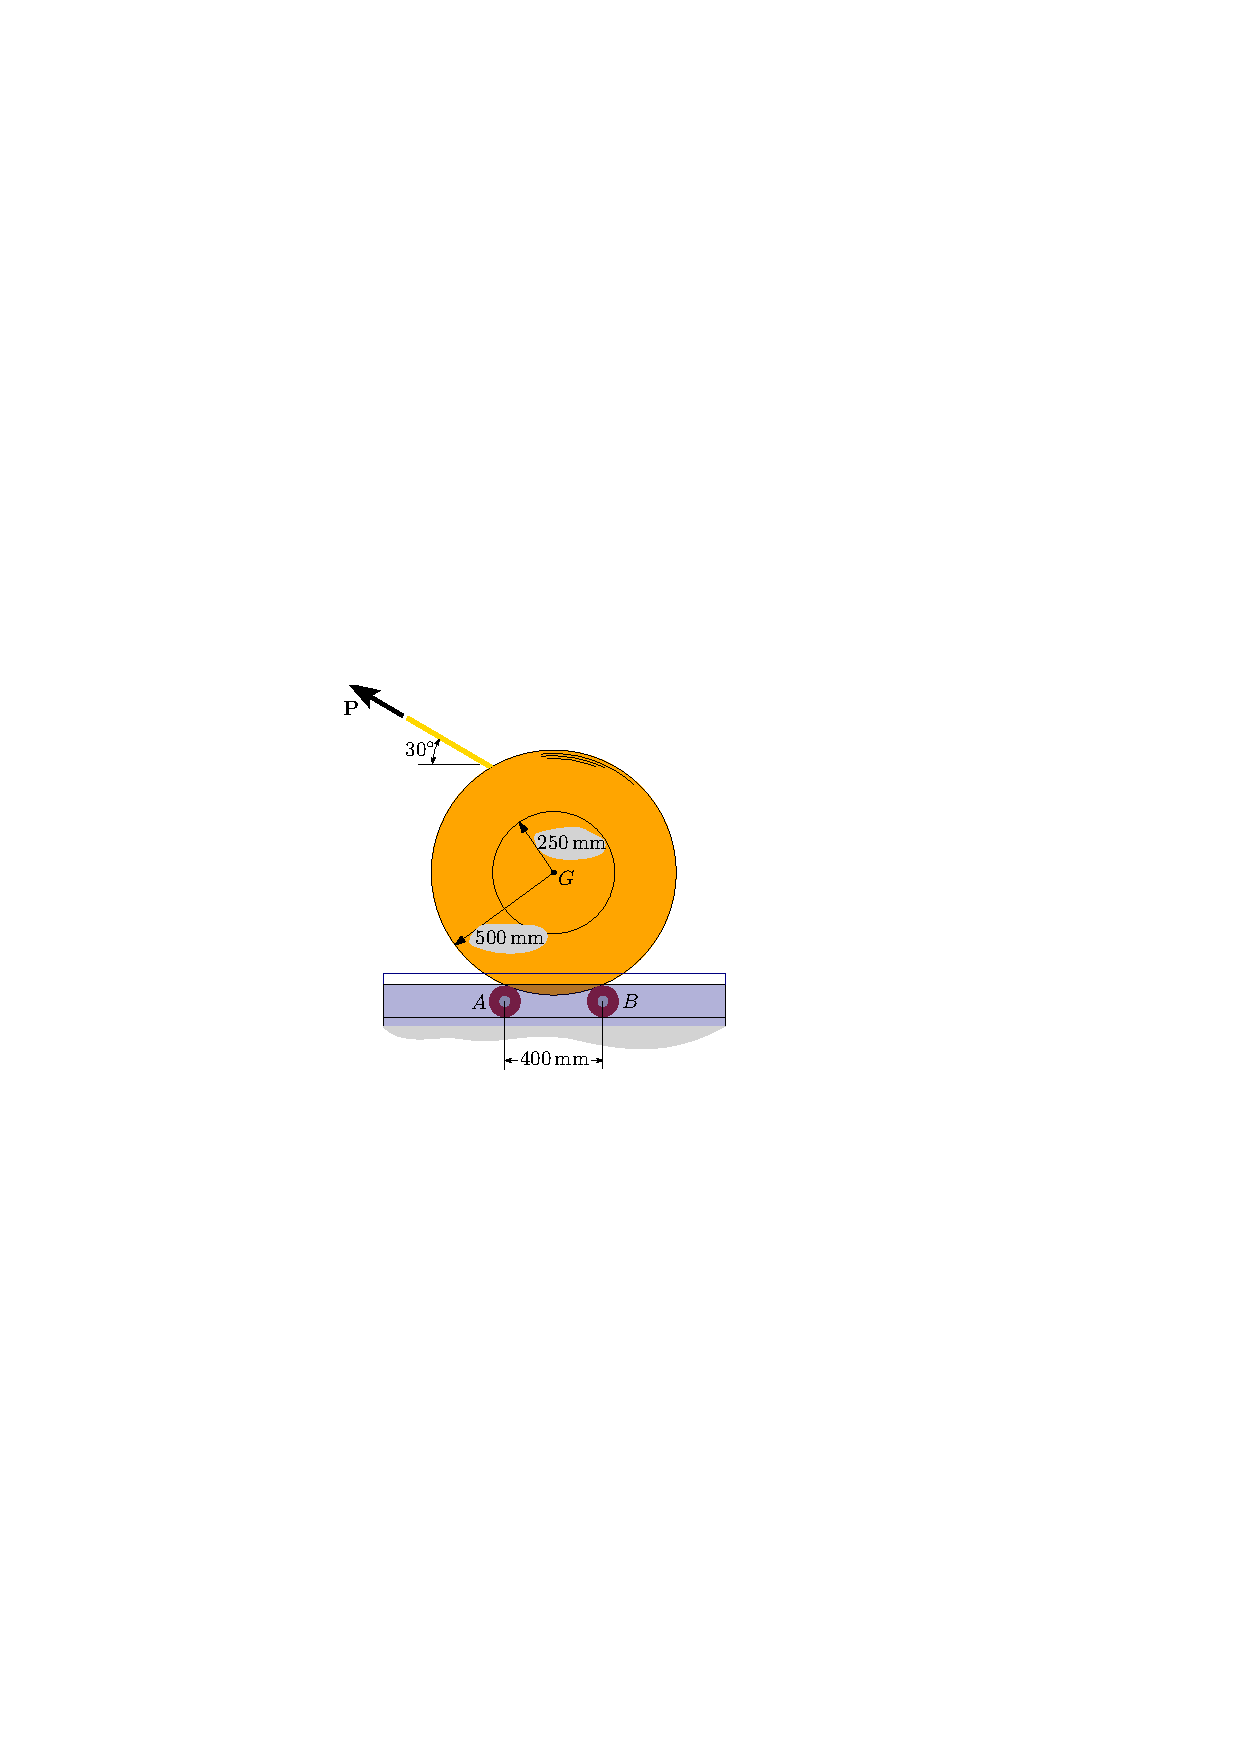
\includegraphics[scale=1.2]{../../images/draw_1_1}
	\end{flushleft}
\end{minipage}
\begin{minipage}{.4\linewidth}
	\item Uma força $P=\SI{20}{\newton}$ é aplicada ao cabo, o qual faz a bobina de \SI{75}{\kilogram} girar sem deslizar sobre os dois rolos, $A$ e $B$, do distribuidor. Determine a velocidade angular da bobina após ela haver completado duas revoluções, partindo do repouso. Despreze a massa do cabo. Cada rolo pode ser considerado um cilindro de \SI{18}{\kilogram}, tendo um raio de \SI{.1}{\meter}. O raio de giração da bobina em relação a seu eixo central é $k_{G}=\SI{.42}{\meter}$.
\end{minipage}